%%
%% This is file `sample-sigplan.tex',
%% generated with the docstrip utility.
%%
%% The original source files were:
%%
%% samples.dtx  (with options: `sigplan')
%% 
%% IMPORTANT NOTICE:
%% 
%% For the copyright see the source file.
%% 
%% Any modified versions of this file must be renamed
%% with new filenames distinct from sample-sigplan.tex.
%% 
%% For distribution of the original source see the terms
%% for copying and modification in the file samples.dtx.
%% 
%% This generated file may be distributed as long as the
%% original source files, as listed above, are part of the
%% same distribution. (The sources need not necessarily be
%% in the same archive or directory.)
%%
%% Commands for TeXCount
%TC:macro \cite [option:text,text]
%TC:macro \citep [option:text,text]
%TC:macro \citet [option:text,text]
%TC:envir table 0 1
%TC:envir table* 0 1
%TC:envir tabular [ignore] word
%TC:envir displaymath 0 word
%TC:envir math 0 word
%TC:envir comment 0 0
%%
%%
%% The first command in your LaTeX source must be the \documentclass command.

\documentclass[sigplan]{acmart}
%% NOTE that a single column version is required for 
%% submission and peer review. This can be done by changing
%% the \doucmentclass[...]{acmart} in this template to 
%% \documentclass[manuscript,screen,review]{acmart}
%% 
%% To ensure 100% compatibility, please check the white list of
%% approved LaTeX packages to be used with the Master Article Template at
%% https://www.acm.org/publications/taps/whitelist-of-latex-packages 
%% before creating your document. The white list page provides 
%% information on how to submit additional LaTeX packages for 
%% review and adoption.
%% Fonts used in the template cannot be substituted; margin 
%% adjustments are not allowed.
%%
%% \BibTeX command to typeset BibTeX logo in the docs
\AtBeginDocument{%
  \providecommand\BibTeX{{%
    \normalfont B\kern-0.5em{\scshape i\kern-0.25em b}\kern-0.8em\TeX}}}

%% Rights management information.  This information is sent to you
%% when you complete the rights form.  These commands have SAMPLE
%% values in them; it is your responsibility as an author to replace
%% the commands and values with those provided to you when you
%% complete the rights form.
%\setcopyright{acmcopyright}
%\copyrightyear{2018}
%\acmYear{2018}
%\acmDOI{XXXXXXX.XXXXXXX}




%%
%% Submission ID.
%% Use this when submitting an article to a sponsored event. You'll
%% receive a unique submission ID from the organizers
%% of the event, and this ID should be used as the parameter to this command.
%%\acmSubmissionID{123-A56-BU3}

%%
%% For managing citations, it is recommended to use bibliography
%% files in BibTeX format.
%%
%% You can then either use BibTeX with the ACM-Reference-Format style,
%% or BibLaTeX with the acmnumeric or acmauthoryear sytles, that include
%% support for advanced citation of software artefact from the
%% biblatex-software package, also separately available on CTAN.
%%
%% Look at the sample-*-biblatex.tex files for templates showcasing
%% the biblatex styles.
%%

%%
%% The majority of ACM publications use numbered citations and
%% references.  The command \citestyle{authoryear} switches to the
%% "author year" style.
%%
%% If you are preparing content for an event
%% sponsored by ACM SIGGRAPH, you must use the "author year" style of
%% citations and references.
%% Uncommenting
%% the next command will enable that style.
%%\citestyle{acmauthoryear}

%%
%% end of the preamble, start of the body of the document source.
\setcopyright{none}%remueve el copyright
\settopmatter{printacmref=false} % remueve la citación
\renewcommand\footnotetextcopyrightpermission[1]{} %remueve el bottom footnote
\begin{document}

%%
%% The "title" command has an optional parameter,
%% allowing the author to define a "short title" to be used in page headers.
\title{Data Profiling}
\subtitle{Calidad de Datos y Big Data en Ingeniería de Software}
%%
%% The "author" command and its associated commands are used to define
%% the authors and their affiliations.
%% Of note is the shared affiliation of the first two authors, and the
%% "authornote" and "authornotemark" commands
%% used to denote shared contribution to the research.
\author{Alejandro Adorjan}
\email{adorjan@ort.edu.uy}
\orcid{0000-0002-5257-284X}



%%
%% By default, the full list of authors will be used in the page
%% headers. Often, this list is too long, and will overlap
%% other information printed in the page headers. This command allows
%% the author to define a more concise list
%% of authors' names for this purpose.
%\renewcommand{\shortauthors}{Trovato and Tobin, et al.}

%%
%% The abstract is a short summary of the work to be presented in the
%% article.
\begin{abstract}
  Abstract
\end{abstract}
\settopmatter{printacmref=false}
%%
%% The code below is generated by the tool at http://dl.acm.org/ccs.cfm.
%% Please copy and paste the code instead of the example below.
%%
%\begin{CCSXML}
%<ccs2012>
% <concept>
%  <concept_id>10010520.10010553.10010562</concept_id>
%  <concept_desc>Computer systems organization~Embedded systems</concept_desc>
%  <concept_significance>500</concept_significance>
% </concept>
% <concept>
%  <concept_id>10010520.10010575.10010755</concept_id>
%  <concept_desc>Computer systems organization~Redundancy</concept_desc>
%  <concept_significance>300</concept_significance>
% </concept>
% <concept>
%  <concept_id>10010520.10010553.10010554</concept_id>
%  <concept_desc>Computer systems organization~Robotics</concept_desc>
%  <concept_significance>100</concept_significance>
% </concept>
% <concept>
%  <concept_id>10003033.10003083.10003095</concept_id>
%  <concept_desc>Networks~Network reliability</concept_desc>
%  <concept_significance>100</concept_significance>
% </concept>
%</ccs2012>
%\end{CCSXML}

%\ccsdesc[500]{Computer systems organization~Embedded systems}
%\ccsdesc[300]{Computer systems organization~Redundancy}
%\ccsdesc{Computer systems organization~Robotics}
%\ccsdesc[100]{Networks~Network reliability}

%%
%% Keywords. The author(s) should pick words that accurately describe
%% the work being presented. Separate the keywords with commas.
\keywords{datasets, neural networks, gaze detection, text tagging}

%% A "teaser" image appears between the author and affiliation
%% information and the body of the document, and typically spans the
%% page.
%\begin{teaserfigure}
 % 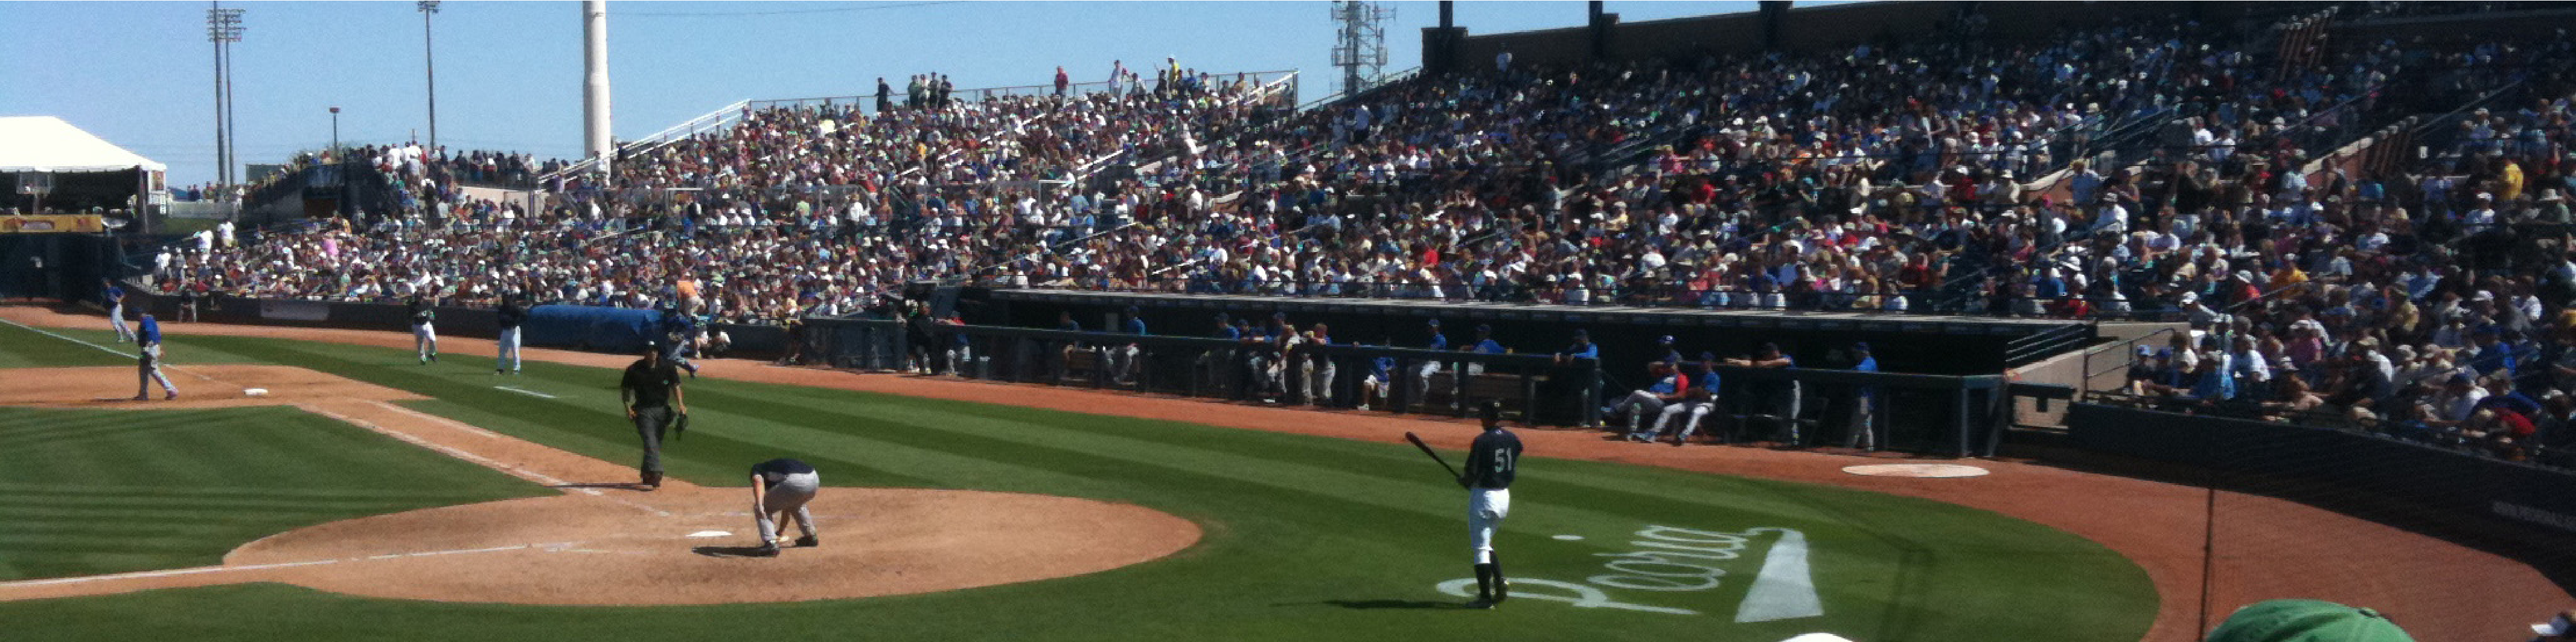
\includegraphics[width=\textwidth]{sampleteaser}
  %\caption{Seattle Mariners at Spring Training, 2010.}
  %\Description{Enjoying the baseball game from the third-base
  %seats. Ichiro Suzuki preparing to bat.}
  %\label{fig:teaser}
%\end{teaserfigure}

%\received{20 February 2007}
%\received[revised]{12 March 2009}
%\received[accepted]{5 June 2009}

%%
%% This command processes the author and affiliation and title
%% information and builds the first part of the formatted document.
\maketitle


\tableofcontents

\section{Objetivo}
El objetivo de este trabajo es realizar un informe respecto de las siguientes tareas: 
\begin{enumerate}
    \item Data profiling de tres archivos de datos publicados.
    \item Especificación de un modelo de calidad de datos que cubra algounos de esos datos. Se deber´priorizar que aspectos y que datos se van a evaluar. Justificación. 
    \item Especificación de la base de datos donde se almacenarán las medidas de calidad obtenidas en la medición. 
    \item Ejecución de la medición de calidad. 
    \item Evaluación final de calidad. Análisis de resultados de medición. Niveles de calidad esperados.
\end{enumerate}

\section{Introducción}

\subsection{Calidad de Datos}
\subsection{Data Profiling}
The process of metadata discovery is known as data profiling. Profiling activities range from ad-hoc approaches, such as eye-balling random subsets of the data or formulating aggregation queries, to systematic inference of structural information and statistics of a dataset using dedicated profiling tools.
\cite{abedjan2017data}. Data profiling is the set of activities and processes to determine the meta- data about a given dataset. Among the simpler results are per-column statistics, such as the number of null values and distinct values in a column, its data type, or the most frequent patterns of its data values. Metadata that are more difficult to compute involve multiple columns, such as inclusion, functional and order dependencies \cite{abedjan2017data}.
The process of metadata discovery is known as data profiling. Profiling activities range from ad-hoc approaches, such as eye-balling random subsets of the data or formulating aggregation queries, to systematic inference of metadata via profiling algorithms \cite{abedjan2018introduction}. Data profiling plays an important role in use cases, such as data exploration, data integration, and data analytics \cite{abedjan2018introduction}. The aim of data Profiling measure data consistency and accuracy, detect data duplications in order to obtain the correct value of data that could be used in decision- making purposes \cite{elbaghazaoui2021data}

\subsection{Modelo de Calidad}

ISO/IEC 25012 - Data Quality model: defines a general data quality model for data retained in a structured format within a computer system. It focuses on the quality of the data as part of a computer system and defines quality characteristics for target data used by humans and systems.

Data Quality model defined in the standard ISO/IEC 25012 is composed of 15 characteristics \url{https://iso25000.com/index.php/en/iso-25000-standards/iso-25012}



\begin{table*}
  \caption{ISO/IEC 25012}
  \label{tab:modelo}
  \begin{tabular}{lp{8cm}}
    \toprule
    Characeristic &Definition\\
    \midrule
    \textbf{Accuracy} &  The degree to which data has attributes that correctly represent the true value of the intended attribute of a concept or event in a specific context of use. \textbf{Syntactic Accuracy:} Syntactic accuracy is defined as the closeness of the data values to a set of values defined in a domain considered syntactically correct.
    \textbf{Semantic Accuracy:} Semantic accuracy is defined as the closeness of the data values to a set of values defined in a domain considered semantically correct.\\
    \textbf{Completeness} & The degree to which subject data associated with an entity has values for all expected attributes and related entity instances in a specific context of use. \\
\textbf{Consistency} & The degree to which data has attributes that are free from contradiction and are coherent with other data in a specific context of use. It can be either or both among data regarding one entity and across similar data for comparable entities.\\
\textbf{Understandability} & The degree to which data has attributes that enable it to be read and interpreted by users, and are expressed in appropriate languages, symbols and units in a specific context of use.
Some information about data understandability are provided by metadata.\\

  \bottomrule
\end{tabular}
\end{table*}


\subsubsection{Dimensions of Quality}


\cite{etcheverry2008qbox}


%\verb|acmconf|}: The default proceedings template style.
% verb|sigchi|}: Used for SIGCHI conference articles.
%\verb|sigchi-a|}: Used for SIGCHI ``Extended Abstract'' articles.
%sigplan|}: Used for SIGPLAN conference articles.
\section{Reporte}

\subsection{Data Profiling de Archivos}

\subsubsection{Fuente de datos}
En el siguiente repositorio 
\href{https://github.com/aadorian/cibse_taller.git}{Repositorio}
estan distonibles todos los fuentes correspondientes al trabajo en particular la ejecución del data profiling está disponible en 
\url{https://bit.ly/softdataprofiling}.

Los metadatos correspondientes asumimos que corresponden a los disponibles en el Ministerio de Turismo
\footnote{https://www.gub.uy/ministerio-turismo/emisivo}
%\url{https://catalogodatos.gub.uy/dataset/ministerio-de-turismo-turismo-emisivo/resource/983ce95a-0c87-467d-8b87-46d3229d0e8a}

\subsubsection{Archivos de Profiling}
Los dataset analizados se encuentran disponibles en el siguiente link:

\url{https://github.com/aadorian/cibse_taller/tree/main/profiling}

\subsection{Categorias del Software de Profiling}

En la Tabla~\ref{tab:sources} se presentan el tipo de alertas de categorias de alertas de profiling provistos por ydata-profiling versión vv4.1.2.
\begin{table}
  \caption{Alertas de ydata-profiling}
  \label{tab:sources}
  \begin{tabular}{ll} 
    \toprule
        Alerta Calidad& Descripción\\
    \midrule
       Constant & Column only contains one value \\
        Zeros &Column only contains zeros \\
        High Correlation & Correlations \\
        High Cardinality & Column > 50 distinct values.\\
        Imbalance  & Column is highly imbalanced \\
        Skewness   & Column’s univariate distribution \\
        Missing Values  & Column has missing values\\
        Infinite Values   &Column has infinite values  \\ 
        Unique Values   & All values of the column are unique\\
         Seasonal &  Column has seasonal pattern\\
          Non Stationary     & Column is a time-series non-stationary\\
        Date   & Column contains data-datetime format \\
          Uniform    & Column follows a uniform distribution\\
          Constant length     & For strings/date/datetimes columns  \\
         Rejected & Variable has mixed types \\
           Unsupported   & Column can’t be analysed\\
            Duplicates   & Dataset-level warning > 10 records\\
    Empty   & Dataset-level warning no data \\
  \bottomrule
\end{tabular}
\end{table}

\subsubsection{Resumen de resultados del DataProfiling}

Los tipos de datos que reconoce ydata-profiling son: Boolean
,Numerical, Categorical, Time-series,
URL,Path,File, Image y  Date (and Datetime).

A continuación se presentan los resultados resumen de la realización de los dataProfiling a las fuentes de datos . 
Para la generación del data profiling se utilizó la versión de ydata-profiling vv4.1.2 \url{https://ydata-profiling.ydata.ai/} que permite realizar el análisis de datos exploratorio 
\url{https://github.com/ydataai/ydata-profiling}.




\url{https://www.gub.uy/ministerio-turismo/datos-y-estadisticas/estadisticas/turismo-emisivo-2022}

Según la normativa uruguaya se entiende por \textit{turismo emisivo} a la actividad turística que realizan los
residentes del país fuera del mismo y por \textit{turismo emisivo} a la actividad turística que realizan los
residentes del país fuera del mismo \url{https://www.impo.com.uy/bases/leyes/19253-2014}.

El t\textit{urismo emisivo} contiene información de residentes en Uruguay con viajes al exterior, gasto y estadía de los mismos por país o destino del viaje, referente a cada trimestre del año\cite{gubemisivo}.
El \textit{turismo receptivo} contiene información correspondientes a los visitantes que ingresaron a Uruguay, gasto y estadía de los mismos, referente a cada trimestre del año.
\cite{gubreceptivo}. 



\subsection{Especificación Modelo de Calidad}


En la Tabla~\ref{tab:modelo} se presentan el modelo de calidad. 
La especificación del modelo de calidad se basa en la propuesta de Etcheverry et. al \cite{etcheverry2008qbox} originalmente basada a su vez en el concepto de GQM (Goal Quality Metrics) propuesto por Basili \cite{basili1992software}.

Etcheverry et. al \cite{etcheverry2008qbox} propone la siguiente categorización.

\begin{itemize}
    \item \textbf{Dimensiones de calidad:} se caracteriza mediante múltiples dimensiones, que ayudan a clasificar los datos. Una dimensión captura un aspecto de alto nivel de la calidad.
    \item \textbf{Factores de calidad}: un factor representa un aspecto particular de una dimensión de calidad, por ejemplo, la precisión de los datos implica corrección semántica, corrección sintáctica y precisión de los datos. Pueden haber varios factores para la misma dimensión; cada factor se adapta mejor a un problema o tipo de sistema en particular.
    \item \textbf{Métricas de calidad: }una métrica es un instrumento utilizado para medir un factor de calidad específico, por ejemplo, el porcentaje de datos del sistema que coinciden con los datos del mundo real es una métrica para la corrección semántica. Pueden haber varias métricas para el mismo factor de calidad.
    \item \textbf{Métodos de calidad:} un método es un proceso que implementa una métrica de calidad. Se definen dos tipos de métodos: (i) métodos de medición, que calculan la calidad de un objeto midiéndolo directamente (por ejemplo, contando el número de valores nulos en una tupla), y (ii) métodos de agregación, que calculan la calidad de un objeto compuesto mediante la agregación de valores de calidad de las partes del objeto (por ejemplo, calcular la precisión de una tabla promediando la precisión de sus tuplas). Pueden haber varios métodos para implementar la misma métrica.

\end{itemize}

Se seleccionarion las siguientes dimensiones

La especificación del modelo cubrirá los datos de \textbf{Operadores}. 
Se evaluaran la dimensión de \textbf{precisión} (Accuracy) y Unicidad. 
Las preguntas a formular en general son relacionadas con 
\begin{itemize}
    \item ¿Estos datos son lo suficientemente precisos para nuestras necesidades?
    \item ¿El nivel de detalle de los datos es adecuado?
    \item ¿Estos datos se corresponden con el mundo real?
    \item ¿Estos datos tienen errores?
    \item ¿El formato de presentación de los datos es correcto? ¿Es estándar?
    
\end{itemize}

Los tres factores a evaluar son : 
    Factor 1: \textbf{Exactitud semántica (Semantic accuracy)}, respondiendo a ¿Los datos se corresponden con la realidad?
Eventualemnte los datos pueden  no corresponden a ningún estado del mundo real y/o a estado equivocado del mundo real y/o  con errores en algunos atributos.
    Factor 2: \textbf{Exactitud sintáctica} \textbf{(Syntactic accuracy)}: respondiendoa ¿Los datos tienen errores sintácticos o de formato?
Eventualmente los datos podrían presentar: 
Errores de valores: Valores fuera de rango, errores ortográficos y de tipeo. 
Errores de estandarización: Valores que no tienen el formato esperado. 
Valores embebidos: Valores que corresponden a múltiples atributos.

El método de medición será calcudo en forma directa midiéndolo directamente
(por ejemplo, contando el número de valores nulos en
una tupla).
    Factor 3: \textbf{Precisión} si los datos tienen el suficiente nivel de detalle

Resumen 

Exactitud semántica: si los datos representan entidades/estados del
 mundo real.
Exactitud sintáctica: si los datos no tienen errores sintácticos.
Precisión: si los datos tienen el suficiente nivel de detalle



Unicidad

Factor: No-duplicación (duplication-free)
Si el dato está duplicado o no, para factor de no-duplicación

Preguntas 
Factores de calidad

\begin{enumerate}
    \item ¿Las categorías de los operadores se corresponden con los que estan regulados por el Ministerio? (Exactitud semántica)
    \item ¿Las direcciones de mail son correctas? (Exactitud sintáctica)
    \item ¿Los telefonos de contacto de los operadores son números válidos? (Exactitud sintáctica)
    \item ¿La geolocalización es precisa ? (Precisión)
\end{enumerate}


En la Tabla~\ref{tab:modelometrica} se presentan los aspectos a evaluar
y en la En la Tabla~\ref{tab:modelometricainstanciada} las métricas intanciadas.

\begin{table*}
  \caption{Modelo de Metricas}
  \label{tab:modelometrica}
  \begin{tabular}{llp{3cm}p{4cm}p{3cm}p{1cm}}
    \toprule
     MetricaID &Dimensión & Factor & Métrica General & Métrica Definición & \\
    \midrule
    M1 & Exactitud & Exactitud sintáctica  & Verificación de Formato  &  granularidad: celda, dominio:{0,1}\\
    M2 & Exactitud& Exactitud semantica  & Diccionario de Datos  &  granularidad: celda, dominio:{0,1}\\
    M3 & Exactitud& Presición & Cantidad Decimales  &  granularidad: columna, dominio:{0,1}\\
    M4 & Unicidad & No-duplicación &  Ratio no-duplicados &  granularidad: tabla, dominio{\%}\\

  \bottomrule
\end{tabular}
\end{table*}

\begin{table*}
  \caption{Metricas Instanciadas }
  \label{tab:modelometricainstanciada}
  \begin{tabular}{lp{4cm}p{5cm}p{7cm}p{1cm}}
    \toprule
         MetricaID &   Metrica Instanciada &  Objetivo\\
    \midrule
       M1 &   Operadores.mail & Verificar que es el formato correcto de email \\
         &   Operadores.web & Verificar que es el formato correcto de url \\
         &   Operadores.telefono & Verificar si la caracteristica corresponde con el Departamento\\
     \midrule
        M2 &   Operadores.tipooperador & Verificar si el operador esta en la lista de operadores clasificadas por el Ministerio de Turismo\\
         &   Operadores.departamento & Verificar si el departamente esta en la lista de departamentos de Uruguay\\ 
      \midrule
        M3 &   Operadores.longitud & Verificar 4 digitos decimales  y > 0 \\
         &   Operadores.latitud & Verificar 4 digitos decimales  y > 0 \\ 
       \midrule
        M4 &   Operadores & Verificar no duplicados.\\
  \bottomrule
\end{tabular}
\end{table*}

\subsection{Especificación de BD de almacenamiento de medidas de Calidad}


\begin{figure*}[h]
  \centering
  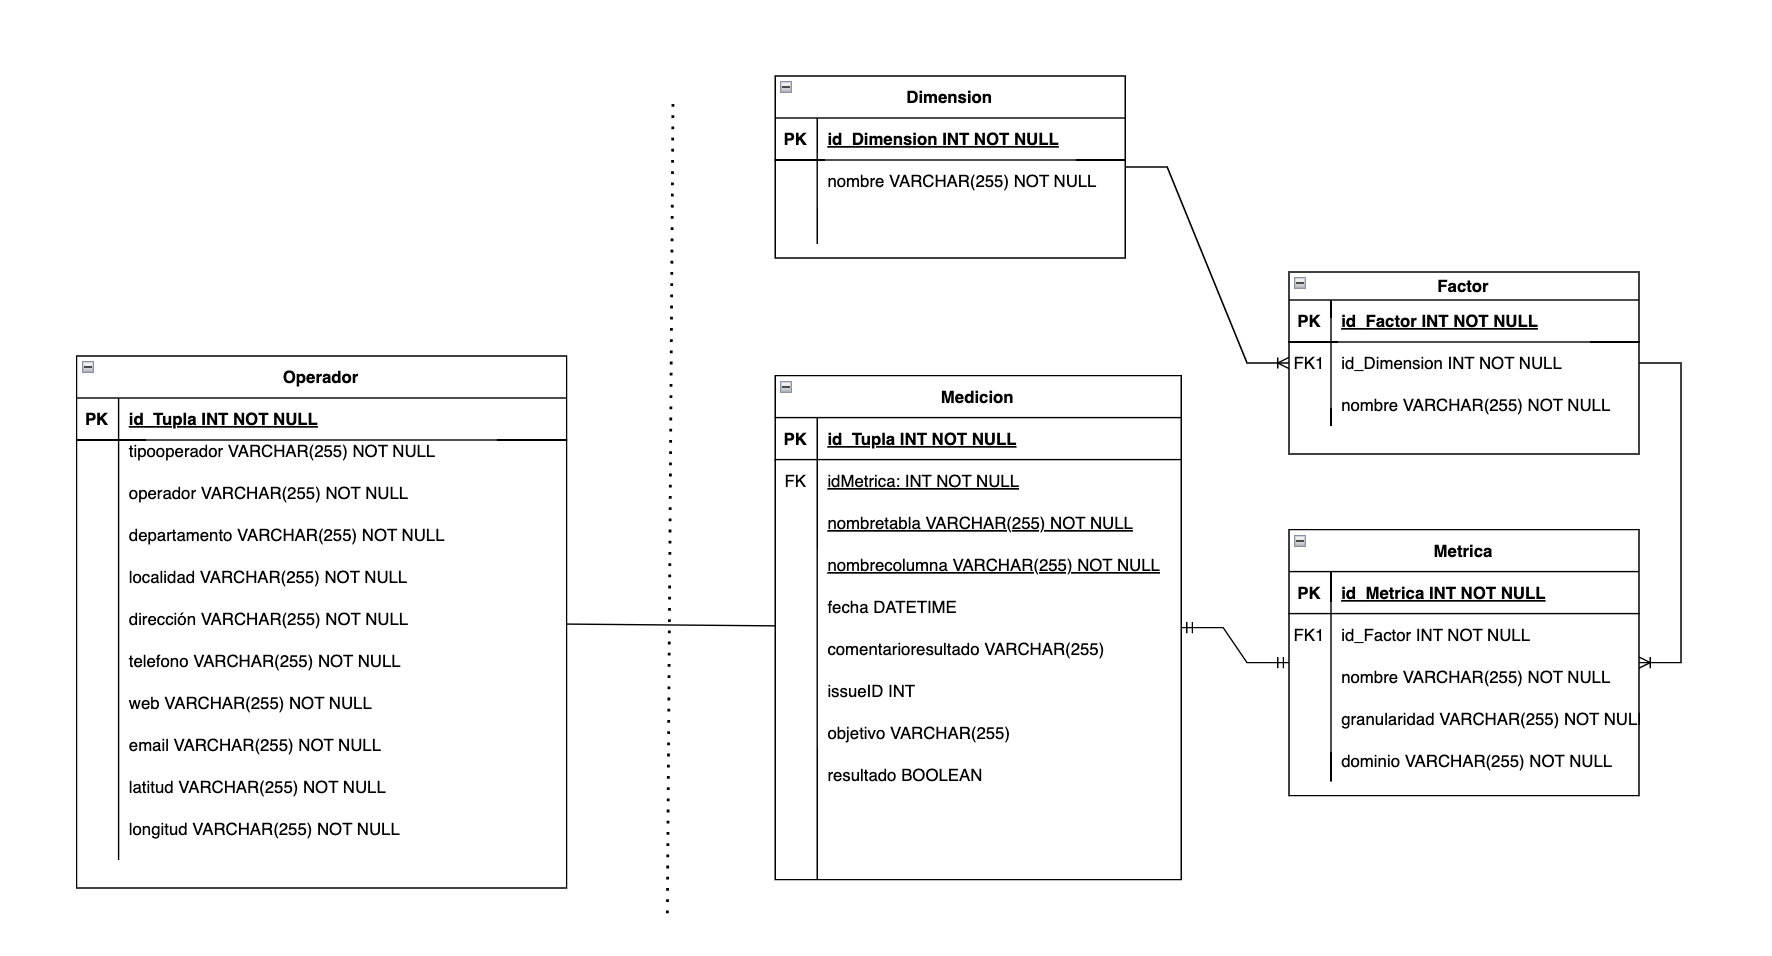
\includegraphics[width=\linewidth]{BD.png}
  \caption{Especificación de diseño de BD de almacenamiento de medidas de calidad obtenidas en la medición} 
  \Description{BD de almacenamiento de medidas de calidad obtenidas en la medición.}
\end{figure*}


\subsection{Ejecución de la medición de Calidad}





\subsection{Evaluación final de la Calidad }




Me pareció interesante evaluar los datos de Operadores  turísticos \footnote{https://www.gub.uy/tramites/inscripcion-operador-turistico} por el hecho de su relevancia en el vínculo entre el turismo receptivo y emisivo.
La actividad de operadores turísticos esta a su vez regulada y con registro de opereradores \url{https://www.gub.uy/tramites/inscripcion-operador-turistico}. 



\section{Tablas}

En la Tabla~\ref{tab:emisivos} se presenta el resumen correspondiente al Data Profiling de Emisivos.

\begin{table}
  \caption{Resumen del Data Profiling de Emisivos}
  \label{tab:emisivos}
  \begin{tabular}{lcl}
    \toprule
    Estadística del dataset&Frecuencia&\\
    \midrule
    Número de variables & 43  \\
    Número de observaciones & 20602  \\
    Celdas faltantes &  7241 \\
    Celdas faltantes (\%)& 0.8\%  \\
    \midrule
    Variables numéricas & 29  \\
    Variables categóricas & 14   \\
    \midrule
    Alertas & 21   \\ 
  \bottomrule
\end{tabular}
\end{table}


\textit{Nota:} Las alertas de la Tabla~\ref{tab:emisivos} corresponden a alta cardinalidad, valores faltantes, ceros y alta varianza.


En la Tabla~\ref{tab:receptivos} se presenta el resumen correspondiente al Data Profiling de Receptivos.

\begin{table}
  \caption{Resumen del Data Profiling de Receptivos}
  \label{tab:receptivos}
  \begin{tabular}{lcl}
    \toprule
    Estadística del dataset&Frecuencia&\\
    \midrule
    Número de variables & 48  \\
    Número de observaciones &  48388 \\
    Celdas faltantes &  	25596 \\
    Celdas faltantes (\%)& \%  	1.1\%\\
    \midrule
    Variables numéricas &  	29 \\
    Variables categóricas &  19  \\
    \midrule
    Alertas &  27  \\ 
  \bottomrule
\end{tabular}
\end{table}

\textit{Nota:} Las alertas de la Tabla~\ref{tab:receptivos} corresponden a alta cardinalidad, desvalance, valores faltantes, ceros y alta varianza.


En la Tabla~\ref{tab:operadores} se presenta el resumen correspondiente al Data Profiling de Operadores Turísticos.

\begin{table}
  \caption{Resumen del Data Profiling de Operadores}
  \label{tab:operadores}
  \begin{tabular}{lcl}
    \toprule
    Estadística del dataset&Frecuencia&\\
    \midrule
    Número de variables &  10 \\
    Número de observaciones & 	3288  \\
    Celdas faltantes &  	1	 \\
    Celdas faltantes (\%)& < 0.1\%\\
    Datos duplicados & 98 \\
    Datos duplicados(\%)& 3.0\% \\
    \midrule
    Variables numéricas &  0	 \\
    Variables categóricas & 10   \\
    \midrule
    Alertas &  11  \\ 
  \bottomrule
\end{tabular}
\end{table}

\textit{Nota:} Las alertas de la Tabla~\ref{tab:operadores} corresponden a alta cardinalidad, duplicados y desvalance.

The ``\verb|figure|'' environment should be used for figures. 

\begin{figure*}[h]
  \centering
  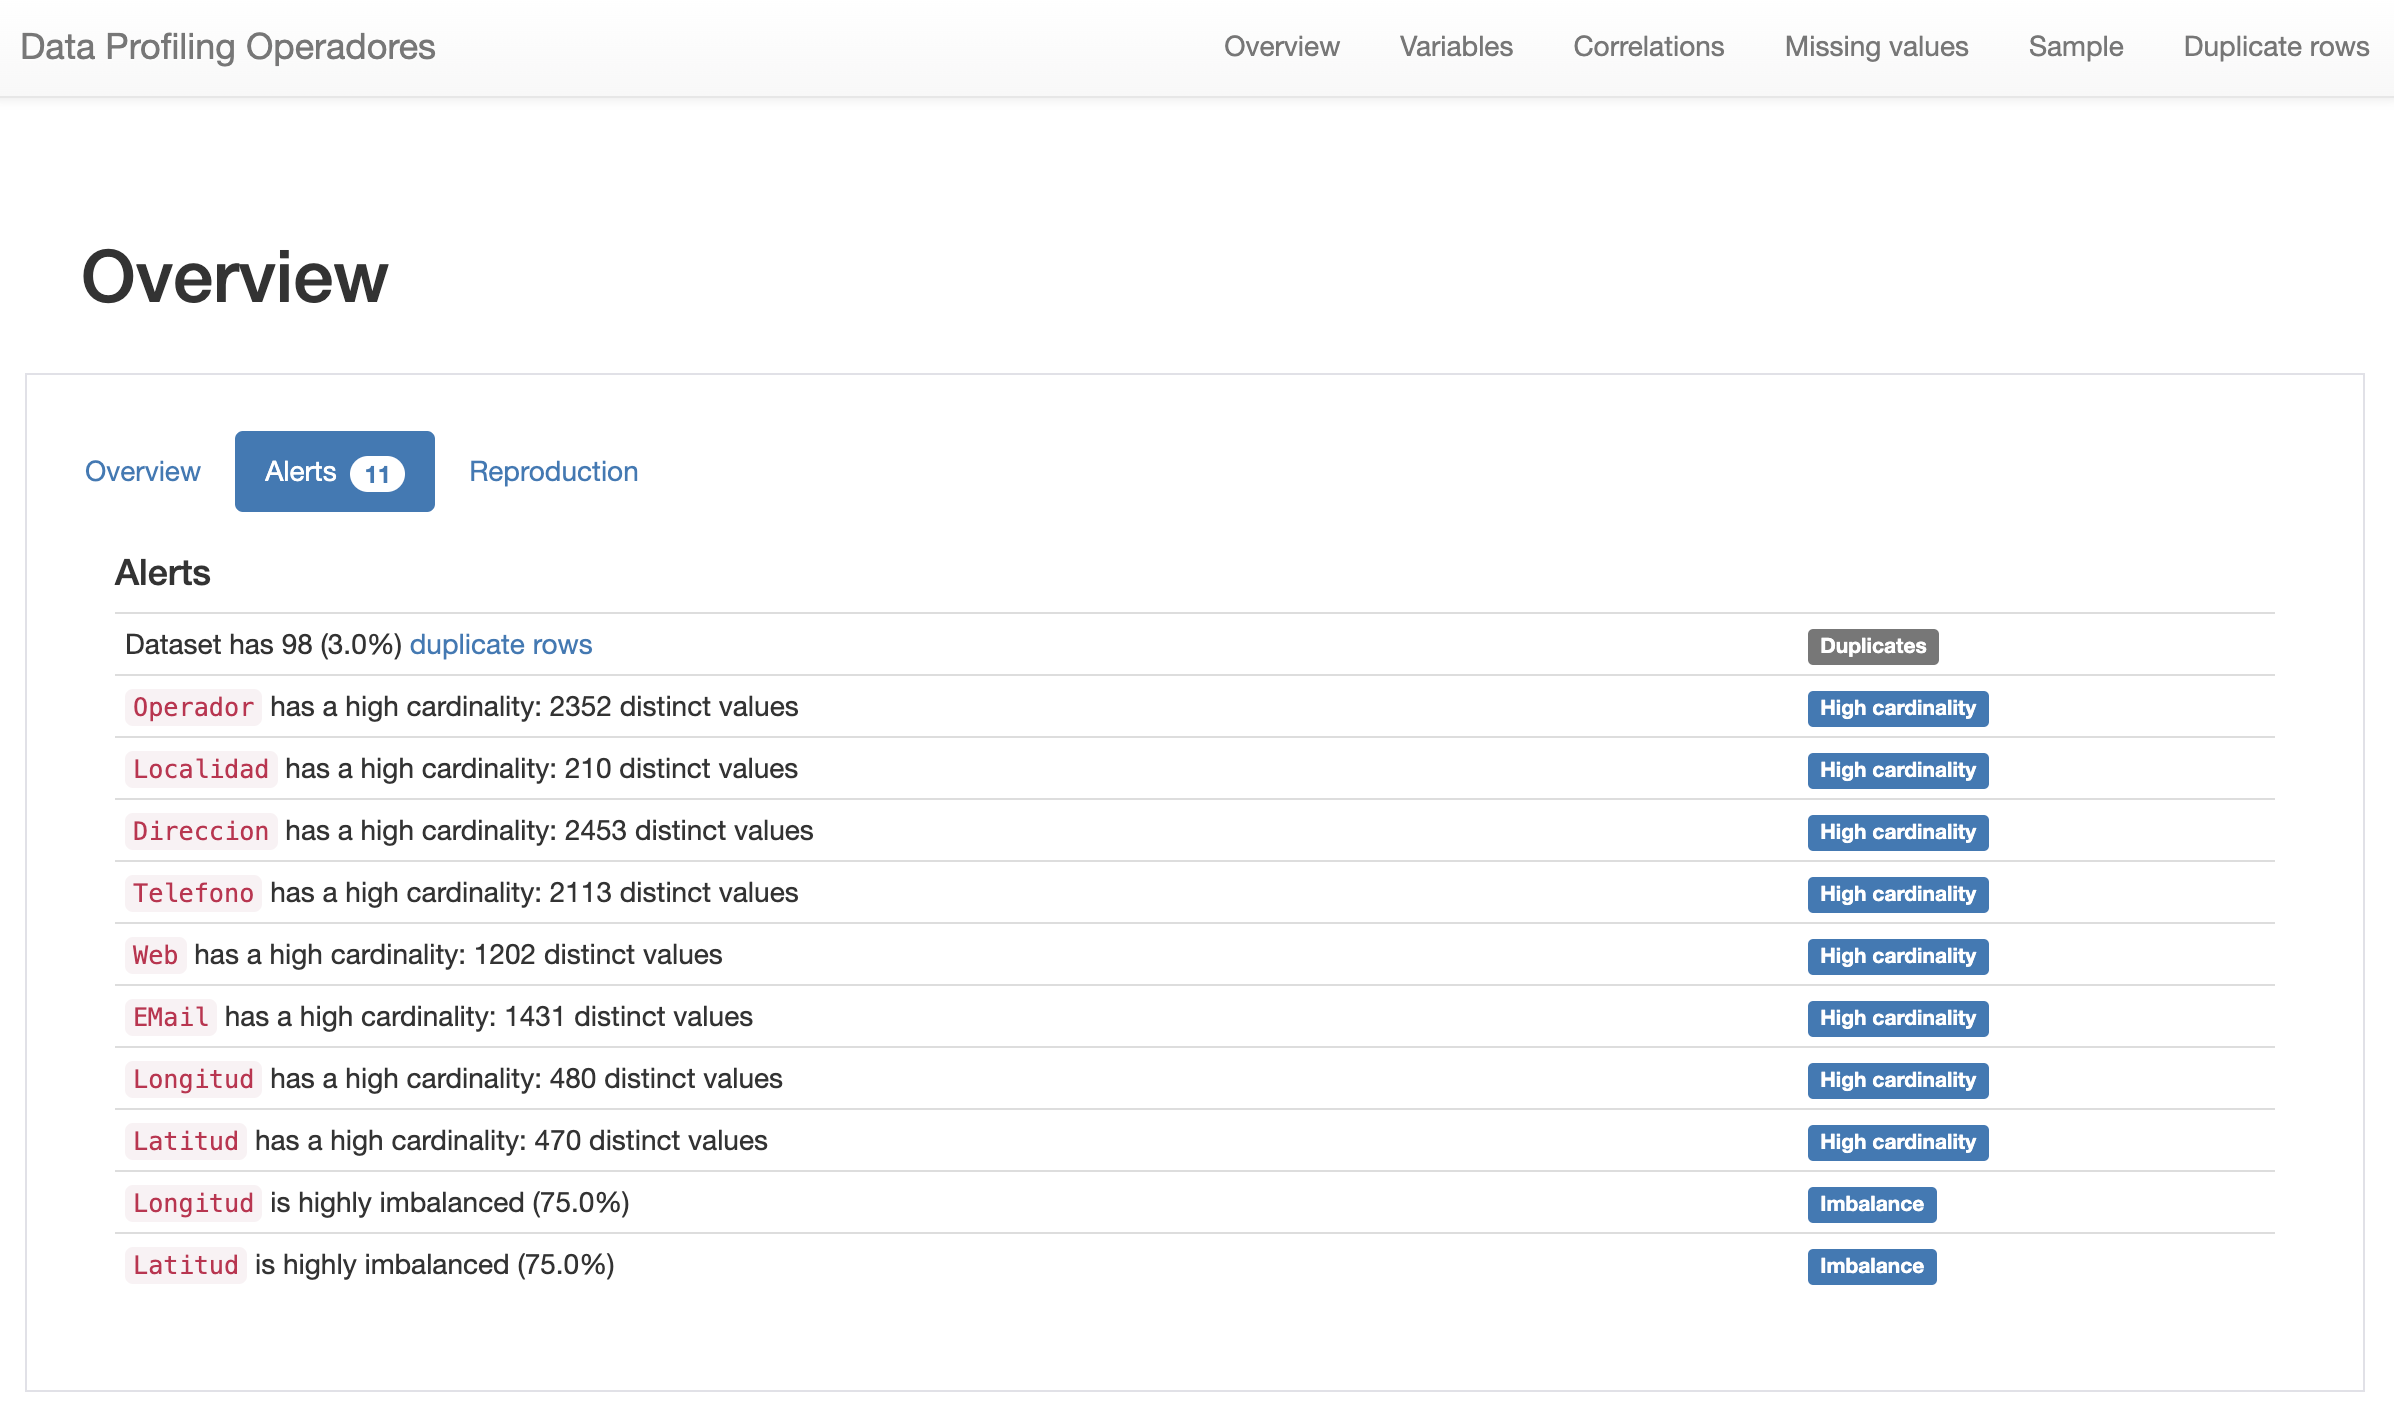
\includegraphics[width=\linewidth]{Overview.png}
  \caption{Overview de Data Profiling Operadores} 
  \Description{A woman and a girl in white dresses sit in an open car.}
\end{figure*}





\begin{table}
  \caption{Tipos }
  \label{tab:operadores}
  \begin{tabular}{lcl}
    \toprule
    Estadística del dataset&Frecuencia&\\
    \midrule
    Número de variables &  10 \\
    Número de observaciones & 	3288  \\
    Celdas faltantes &  	1	 \\
    Celdas faltantes (\%)& < 0.1\%\\
    Datos duplicados & 98 \\
    Datos duplicados(\%)& 3.0\% \\
    \midrule
    Variables numéricas &  0	 \\
    Variables categóricas & 10   \\
    \midrule
    Alertas &  11  \\ 
  \bottomrule
\end{tabular}
\end{table}

\section{Diseño}

\begin{figure*}[h]
  \centering
  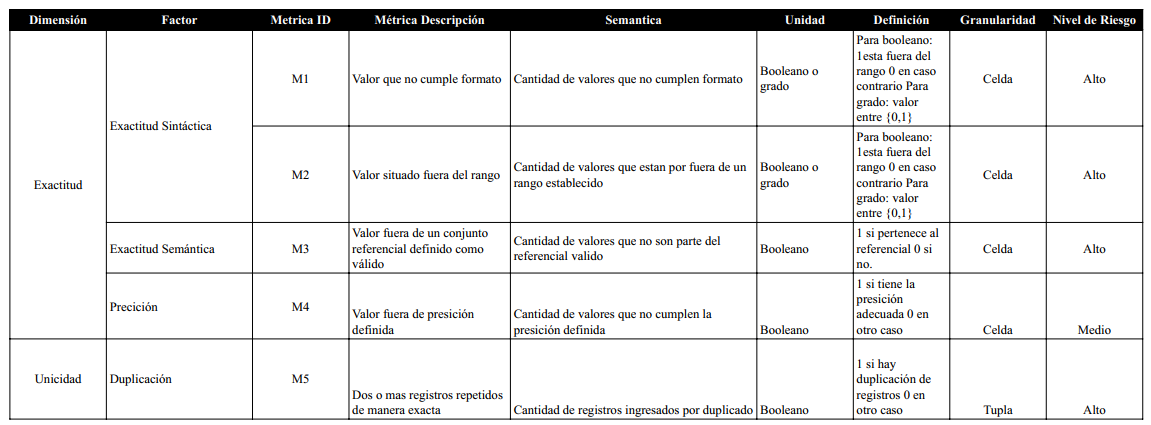
\includegraphics[width=\linewidth]{1.png}
  \caption{Especificación de Registro } 
  \Description{Especificación de Registro del Data Profiling.}
\end{figure*}

\begin{figure*}[h]
  \centering
  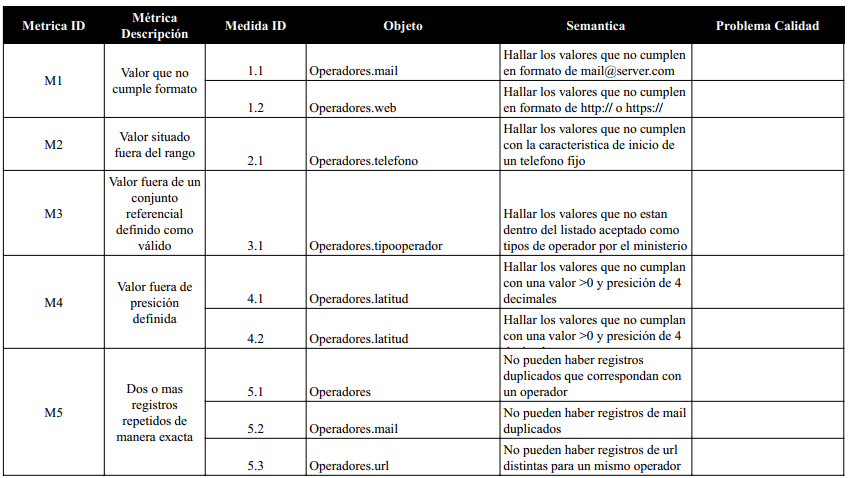
\includegraphics[width=\linewidth]{2.png}
  \caption{Registro de Metricas} 
  \Description{Registro de Metricas .}
\end{figure*}


\begin{figure*}[h]
  \centering
  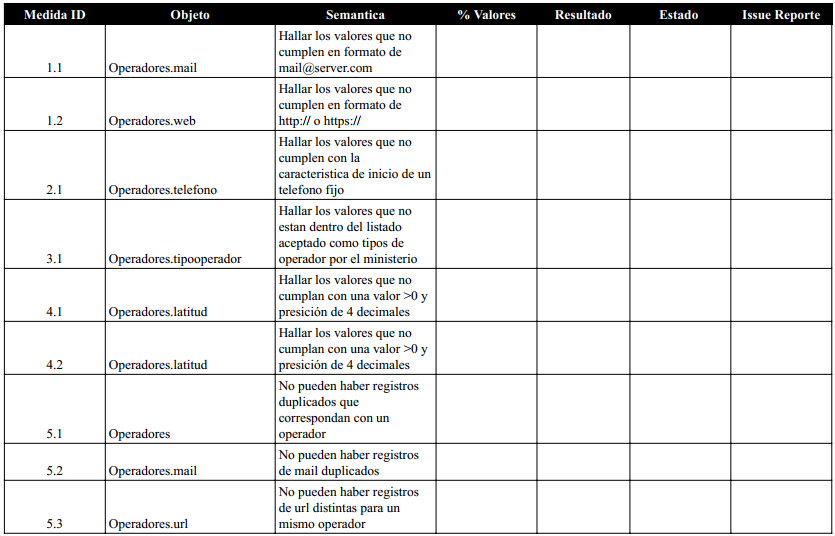
\includegraphics[width=\linewidth]{3.png}
  \caption{Template de registro de ejecución } 
  \Description{emplate de registro de ejecución.}
\end{figure*}


\section{Resultados}

Los tipos de Operadores validados por parte del Ministerio de Turimo de Uruguay son 10 : 
agencia de viajes, transporte turístico, alojamiento turístico, prestadores de servicios turísticos inmobiliarios, turismo aventura, establecimiento enológico (prestan servicios de alojamiento), establecimiento enológico (no prestan servicios de alojamiento), sucursal, guía de turismo, organizadores profesionales de congresos, observación de cetáceos, arrendadora de vehículos sin conductor, prestadores de servicios turísticos rurales, salas de convenciones instaladas en establecimientos rurales, salas de convenciones instaladas en alojamientos turísticos, salas de convenciones instaladas en establecimientos que no requieren inscripción en el registro de prestadores de servicios turísticos.
Fuente: \url{https://www.gub.uy/tramites/inscripcion-operador-turistico}




\section{Resumen Ejecución}

   \begin{table}
  \caption{Ejecución}
  \label{tab:ejecución}
  \begin{tabular}{lcl}
    \toprule
    Dimension&Factor&Metrica\\
    \midrule
    Número de variables &  10 \\

  \bottomrule
\end{tabular}
\end{table}




      

\section{Conclusion}

%%
%% The acknowledgments section is defined using the "acks" environment
%% (and NOT an unnumbered section). This ensures the proper
%% identification of the section in the article metadata, and the
%% consistent spelling of the heading.
\begin{acks}
To Robert, for the bagels and explaining CMYK and color spaces.
\end{acks}

%%
%% The next two lines define the bibliography style to be used, and
%% the bibliography file.
\bibliographystyle{ACM-Reference-Format}
\bibliography{sample-base}

%%
%% If your work has an appendix, this is the place to put it.
\appendix

\end{document}
\endinput
%%
%% End of file `sample-sigplan.tex'.
